\documentclass{article}
\usepackage[margin=1in]{geometry}
\usepackage{amsmath,amsthm,amssymb}
\usepackage{bbm,enumerate,mathtools}
\usepackage{tikz,pgfplots}
\usepackage{chessboard}
\usepackage[hidelinks]{hyperref}
\usepackage{multicol} % Problem 35
\usepackage{xstring} % Difficulty command
\usetikzlibrary{shapes.geometric}

\newenvironment{question}{\begin{trivlist}\item[\textbf{Question.}]}{\end{trivlist}}
\newenvironment{note}{\begin{trivlist}\item[\textbf{Note.}]}{\end{trivlist}}
\newenvironment{references}{\begin{trivlist}\item[\textbf{References.}]}{\end{trivlist}}
\newenvironment{related}{\begin{trivlist}\item[\textbf{Related.}]\end{trivlist}\begin{enumerate}}{\end{enumerate}}

\newcommand\score[1]{
\pgfmathsetmacro\pgfxa{#1+1}
\tikzstyle{scorestars}=[
  star,
  star points=5,
  star point ratio=2.25,
  draw,
  inner sep=3pt,
  anchor=outer point 5
]
  \begin{tikzpicture}[baseline]
    \draw[opacity=0] (0,-0.5) rectangle (0,0.2); % Workaround for whitespace at the bottom.
    \foreach \i in {1,...,4} {
      \pgfmathparse{(\i<=#1?"yellow":"gray")}
      \edef\starcolor{\pgfmathresult}
      \draw (\i*4.5ex,0) node[name=star\i,scorestars,fill=\starcolor]  {};
    }
  \end{tikzpicture}
}

\newcommand{\difficulty}[1]{%
  \IfEqCase{#1}{%
      {1}{
        
\begin{tikzpicture}[scale=0.7, baseline=0.9mm]%
          \definecolor{slopegreen}{rgb}{0.0, 0.5, 0.0}%
          \fill[slopegreen] (0.5,0.5) circle (0.5);%
        \end{tikzpicture}%
      }%
      {2}{
        
\begin{tikzpicture}[scale=0.7, baseline=0.9mm]%
          \definecolor{slopeblue}{rgb}{0.0, 0.44, 1.00}
          \fill[slopeblue] (0,0) rectangle (1,1);%
        \end{tikzpicture}%
      }%
      {3}{
\begin{tikzpicture}[scale=0.7, baseline=0.9mm]\fill (0,0.5)--(0.5, 0)--(1,0.5)--(0.5,1)--cycle; \end{tikzpicture}}%
      {4}{
\begin{tikzpicture}[scale=0.7, baseline=0.9mm]\fill (0.25,0)--(0,0.5)--(0.25,1)--(0.5,0.5)--cycle; \fill (0.75,0)--(0.5,0.5)--(0.75,1)--(1,0.5)--cycle;\end{tikzpicture}}%
      % you can add more cases here as desired
  }[\PackageError{difficulty}{Undefined difficulty level: #1}{}]%
}%
\newcommand{\rating}[2]{\difficulty{#1}\\\score{#2}\\}

\usetikzlibrary{patterns}

\begin{document}
\rating{3}{3}
  Suppose you have two finite groups $G$ and $H$, and a $H$-set $\Omega$.
  Denote the base of the wreath product of $G$ by $H$ as $
    K = \prod_{\omega \in \Omega} g_\omega.
  $

  We're interested in determining when it is possible to construct a finite
  sequence, $\{k_i \in K\}_{i=1}^N$, such that for any choice of
  $\alpha \in G \wr_\Omega H$ and any sequence $\{h_i \in H\}_{i=1}^N$,
  there exists $n \leq N$ satisfying \[
    \alpha \cdot (k_1, h_1) \cdot (k_2, h_2) \cdots (k_n, h_n) = (e_K, h)
  \] for some $h \in H$.
\begin{figure}[ht!]
  \centering
  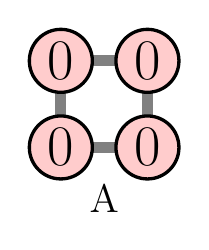
\begin{tikzpicture}
    \draw[gray, line width=4] (0.45,0.45) rectangle (1.55,1.55);
    \draw[very thick, fill=red!20]
      (0.45, 0.45) circle (0.4) node {\huge 0}
      (1.55, 0.45) circle (0.4) node {\huge 0}
      (0.45, 1.55) circle (0.4) node {\huge 0}
      (1.55, 1.55) circle (0.4) node {\huge 0};
    \node at (1, -0.2) {\Large A};
  \end{tikzpicture}
  \hspace{0.5cm}
  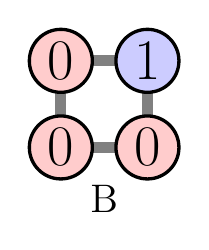
\begin{tikzpicture}
    \draw[gray, line width=4] (0.45,0.45) rectangle (1.55,1.55);
    \draw[very thick, fill=red!20]
      (0.45, 0.45) circle (0.4) node {\huge 0}
      (1.55, 0.45) circle (0.4) node {\huge 0}
      (0.45, 1.55) circle (0.4) node {\huge 0};
    \draw[very thick, fill=blue!20]
      (1.55, 1.55) circle (0.4) node {\huge 1};

    \node at (1, -0.2) {\Large B};
  \end{tikzpicture}
  \hspace{0.5cm}
  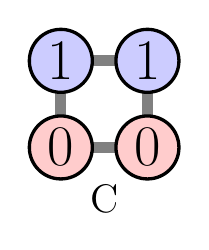
\begin{tikzpicture}
    \draw[gray, line width=4] (0.45,0.45) rectangle (1.55,1.55);
    \draw[very thick, fill=red!20]
      (0.45, 0.45) circle (0.4) node {\huge 0}
      (1.55, 0.45) circle (0.4) node {\huge 0};
    \draw[very thick, fill=blue!20]
      (0.45, 1.55) circle (0.4) node {\huge 1}
      (1.55, 1.55) circle (0.4) node {\huge 1};

    \node at (1, -0.2) {\Large C};
  \end{tikzpicture}
  \hspace{0.5cm}
  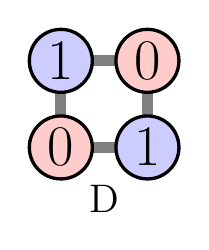
\begin{tikzpicture}
    \draw[gray, line width=4] (0.45,0.45) rectangle (1.55,1.55);
    \draw[very thick, fill=red!20]
      (0.45, 0.45) circle (0.4) node {\huge 0}
      (1.55, 1.55) circle (0.4) node {\huge 0};
    \draw[very thick, fill=blue!20]
      (1.55, 0.45) circle (0.4) node {\huge 1}
      (0.45, 1.55) circle (0.4) node {\huge 1};

    \node at (1, -0.2) {\Large D};
  \end{tikzpicture}
  \\
  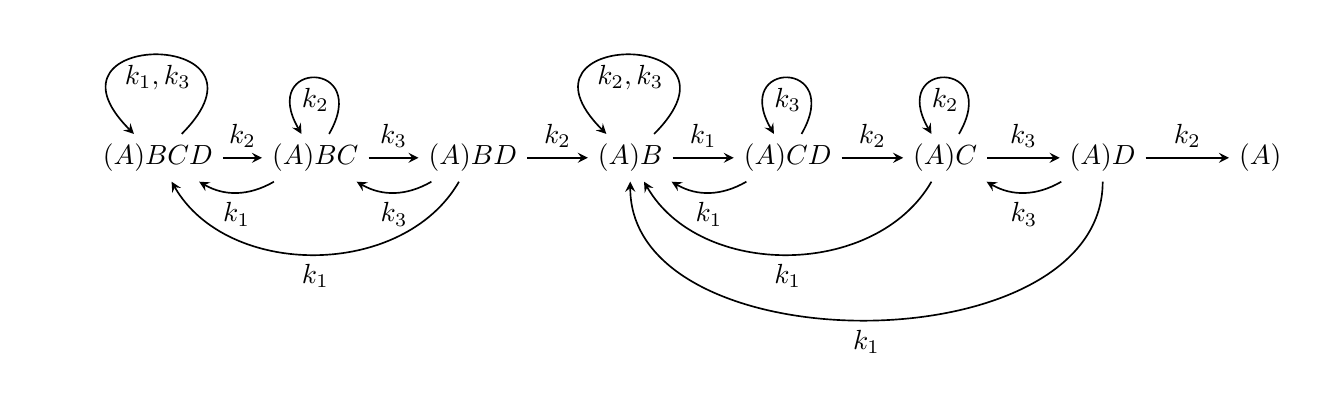
\begin{tikzpicture}[
    > = stealth, % arrow head style
    auto,
    node distance = 2cm, % distance between nodes
    semithick % line style
  ]
    \node (a) {$(A)BCD$};
    \node (b) [right of=a] {$(A)BC$};
    \node (c) [right of=b] {$(A)BD$};
    \node (d) [right of=c] {$(A)B$};
    \node (e) [right of=d] {$(A)CD$};
    \node (f) [right of=e] {$(A)C$};
    \node (g) [right of=f] {$(A)D$};
    \node (h) [right of=g] {$(A)$};

    \draw[looseness=8,out=45,in=135,->] (a) edge node {$k_1,k_3$} (a);
    \draw[->] (a) edge node {$k_2$} (b);
    \draw[->] (b) edge node {$k_3$} (c);
    \draw[->] (c) edge node {$k_2$} (d);
    \draw[->] (d) edge node {$k_1$} (e);
    \draw[->] (e) edge node {$k_2$} (f);
    \draw[->] (f) edge node {$k_3$} (g);
    \draw[->] (g) edge node {$k_2$} (h);

    \draw[looseness=8,out=60,in=120,->] (b) edge node {$k_2$} (b);
    \draw[looseness=1,out=210,in=330,->] (b) edge node {$k_1$} (a);

    \draw[looseness=1,out=240,in=300,->] (c) edge node {$k_1$} (a);
    \draw[looseness=1,out=210,in=330,->] (c) edge node {$k_3$} (b);

    \draw[looseness=8,out=45,in=135,->] (d) edge node {$k_2,k_3$} (d);

    \draw[looseness=1,out=210,in=330,->] (e) edge node {$k_1$} (d);
    \draw[looseness=8,out=60,in=120,->] (e) edge node {$k_3$} (e);

    \draw[looseness=8,out=60,in=120,->] (f) edge node {$k_2$} (f);
    \draw[looseness=1,out=240,in=300,->] (f) edge node {$k_1$} (d);

    \draw[looseness=1,out=210,in=330,->] (g) edge node {$k_3$} (f);
    \draw[looseness=1,out=270,in=270,->] (g) edge node {$k_1$} (d);
  \end{tikzpicture}
  \caption[]{
    Suppose $G = \mathbb{Z}_2$, $H = C_4$, and $\Omega$ is the rotations of the
    square, with $H$ acting in the ordinary way. Moreover, suppose that
    $k_0 = (1,1,1,1)$, $k_1 = (1,0,0,0)$, $k_2 = (1,0,1,0)$, and
    $k_3 = (1,1,0,0)$. Then the sequence
    $(k_0, k_2, k_0, k_3, k_0, k_2, k_0, k_1, k_0, k_2, k_0, k_3, k_0, k_2, k_0)$
    satisfies the above condition.
    % Let $X$ be the vertices of the square $G = C_4$ the cyclic group which acts
    % on the $X$ by rotation, $H = \mathbb Z_2$, and $t(x) \equiv 0$.
    % Then interspersing the above sequence of $N=7$ moves with $f(x) = 1$ will
    % always result in the sequence reaching the target function, where $1, 2,$
    % and $3$ are the moves that flip one coin, two opposite coins, and
    % two adjacent coins respectively.
  }
\end{figure}
\begin{question}
  What conditions on $G \wr_\Omega H$ guarantee such a finite sequence of
  elements in $K$?
\end{question}

\begin{related}
  \item Given $G \wr_\Omega H$, what is $N$, the minimum length of the sequence?
  \item If both $\alpha$ and the sequence $\{h_i \in H\}_{i=1}^N$ are chosen
  uniformly at random, what is the expected value of the minimal $n$ such that $
    \alpha \cdot (k_1, h_1) \cdot (k_2, h_2) \cdot \dots \cdot (k_n, h_n) = (e, k)
  $?
  \item What if there is a set of elements in the base, any one of which is valid.
  (e.g. all sets satisfying the condition that the number of heads is congruent
  to $2 \pmod 3$.)
  \item What if something about $s_i$ is told to you after the $i$th move for each
    $i$ (and the strategy can depend on this information)?
\end{related}
\begin{note}
  This problem appears in \href{Peter Winkler's book}{} under the name
  ``Spinning Switches''.
  The can be generalized to $H = C_{2^n}$ and $\Omega$ a $2^n$-gon,
  but no other $m$-gon.
  The idea is that (1) you can't solve any $m$-gon with $m$ odd, and (2) you
  can solve a $m$-gon if and only if you can solve a $d$-gon for every proper
  divisor $d \mid m$.
  If you allow ``coins'' to have three states, then you can solve this on a
  $3^n$-gon.
\end{note}

\begin{references}
  \item \url{http://mathriddles.williams.edu/?p=77}
  \item \url{https://mathoverflow.net/q/332600/104733}
  \item \url{https://en.wikipedia.org/wiki/Four_glasses_puzzle}
\end{references}
\end{document}
